% !TeX root = RJwrapper.tex
\title{Changes on CRAN}

\subtitle{%
2024-01-01 to 2024-06-30
}

\author{by Kurt Hornik, Uwe Ligges, and Achim Zeileis}

\maketitle


\section{CRAN growth}\label{cran-growth}

In the past 6 months, 1060~new packages were
added to the CRAN package repository. 405~packages
were unarchived, 690~were archived and
7~had to be removed. The following shows the
growth of the number of active packages in the CRAN package repository:

\begin{center}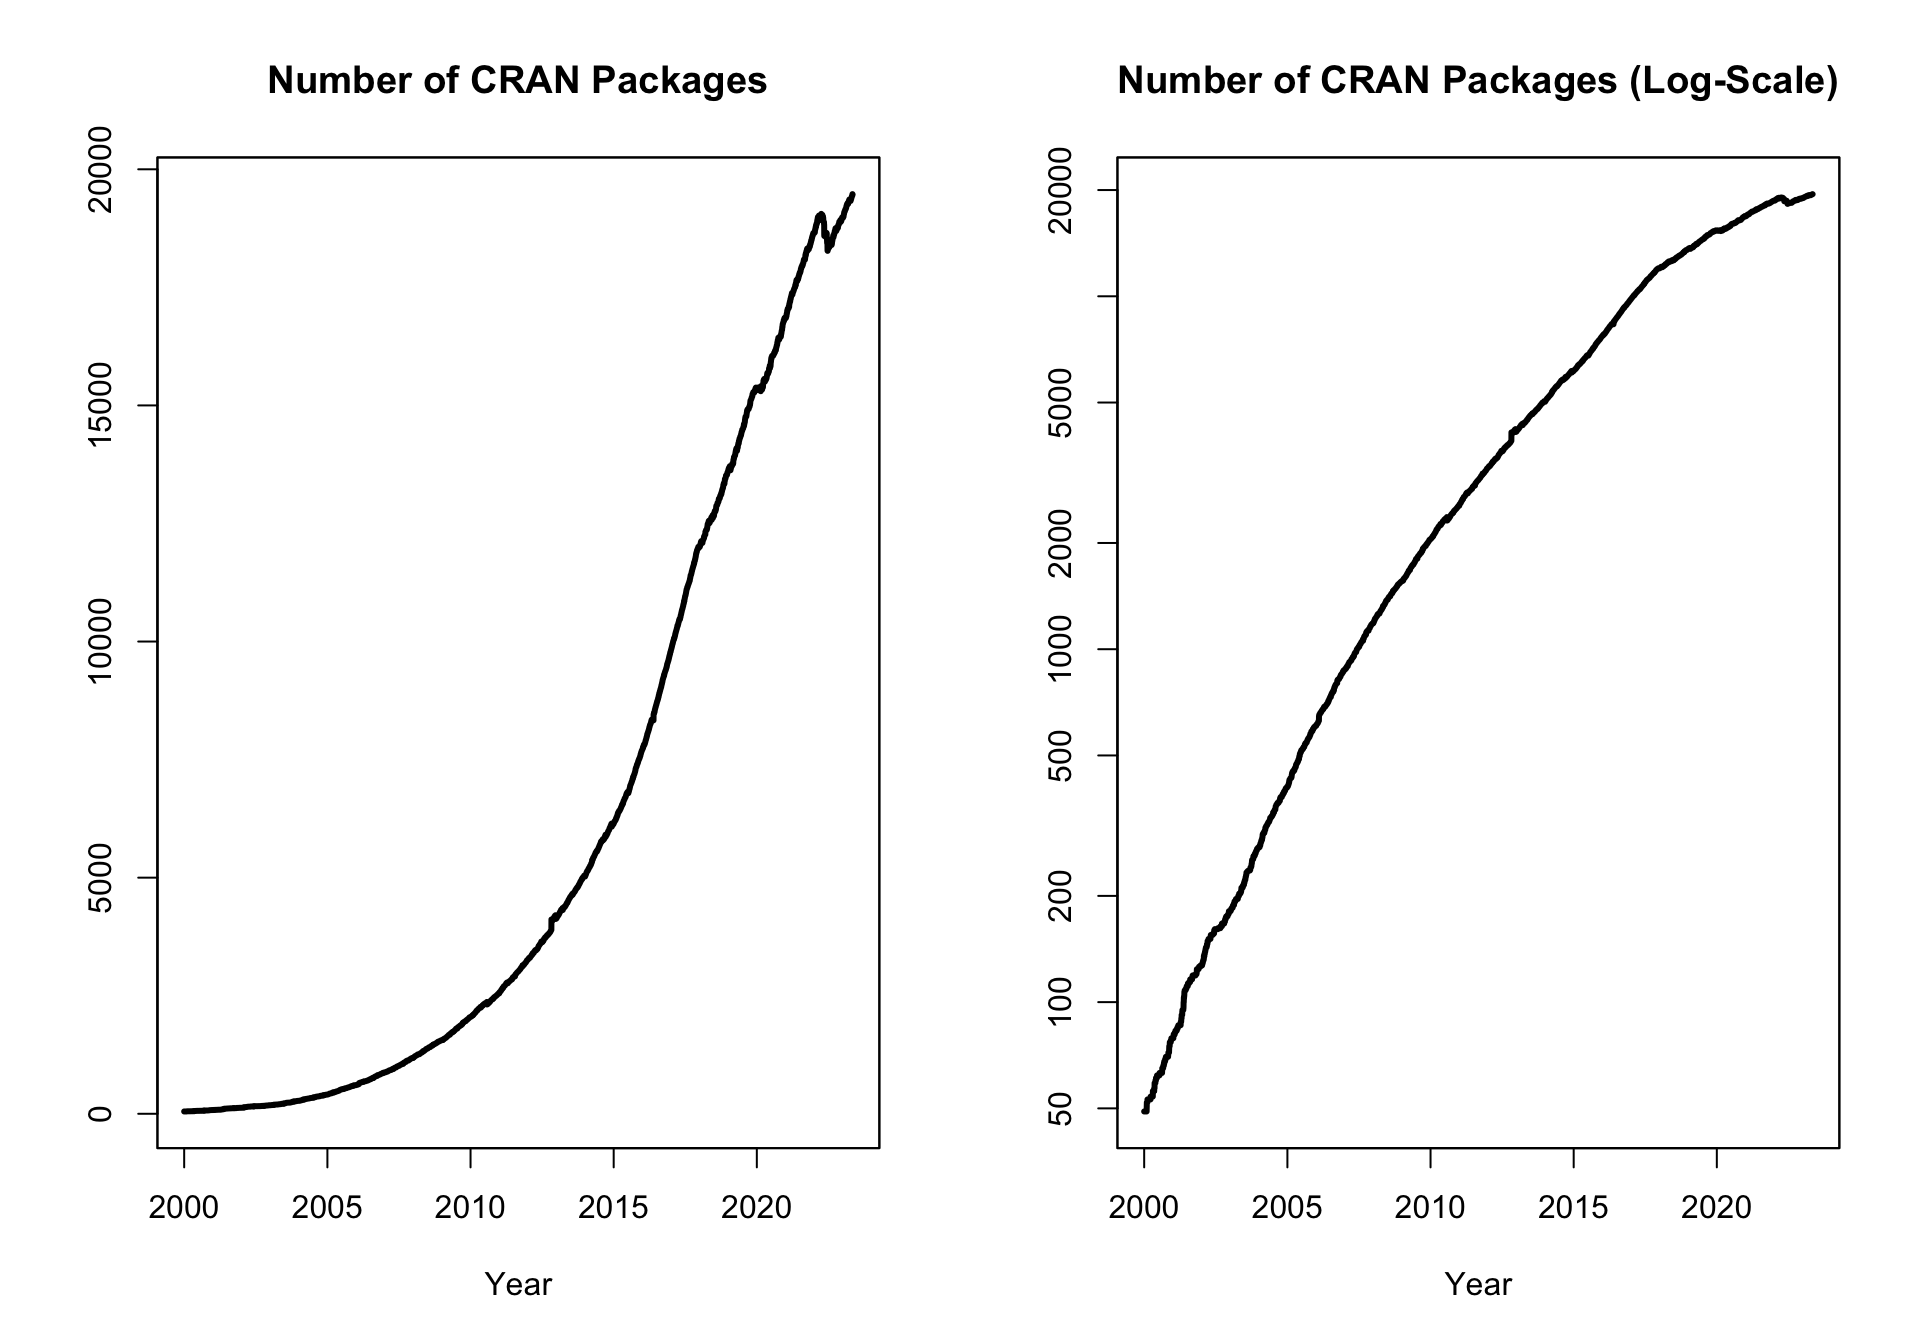
\includegraphics[width=1\linewidth,alt={CRAN growth: Number of CRAN packages over time in levels (left) and in logs (right).}]{RJ-2024-1-cran_files/figure-latex/cran_growth-1} \end{center}

\noindent On 2024-06-30, the number of active packages was around~21018.

\section{CRAN package submissions}\label{cran-package-submissions}

From January 2024 to June 2024
CRAN received 14584~package submissions.
For these, 23887~actions took place of which
16756~(70\%) were auto processed actions and
7131~(30\%) manual actions.

Minus some special cases, a summary of the auto-processed and manually
triggered actions follows:

\begin{longtable}[]{@{}
  >{\raggedright\arraybackslash}p{(\columnwidth - 16\tabcolsep) * \real{0.0986}}
  >{\raggedleft\arraybackslash}p{(\columnwidth - 16\tabcolsep) * \real{0.1127}}
  >{\raggedleft\arraybackslash}p{(\columnwidth - 16\tabcolsep) * \real{0.1127}}
  >{\raggedleft\arraybackslash}p{(\columnwidth - 16\tabcolsep) * \real{0.1127}}
  >{\raggedleft\arraybackslash}p{(\columnwidth - 16\tabcolsep) * \real{0.1127}}
  >{\raggedleft\arraybackslash}p{(\columnwidth - 16\tabcolsep) * \real{0.1127}}
  >{\raggedleft\arraybackslash}p{(\columnwidth - 16\tabcolsep) * \real{0.1127}}
  >{\raggedleft\arraybackslash}p{(\columnwidth - 16\tabcolsep) * \real{0.1127}}
  >{\raggedleft\arraybackslash}p{(\columnwidth - 16\tabcolsep) * \real{0.1127}}@{}}
\toprule\noalign{}
\begin{minipage}[b]{\linewidth}\raggedright
\end{minipage} & \begin{minipage}[b]{\linewidth}\raggedleft
archive
\end{minipage} & \begin{minipage}[b]{\linewidth}\raggedleft
inspect
\end{minipage} & \begin{minipage}[b]{\linewidth}\raggedleft
newbies
\end{minipage} & \begin{minipage}[b]{\linewidth}\raggedleft
pending
\end{minipage} & \begin{minipage}[b]{\linewidth}\raggedleft
pretest
\end{minipage} & \begin{minipage}[b]{\linewidth}\raggedleft
publish
\end{minipage} & \begin{minipage}[b]{\linewidth}\raggedleft
recheck
\end{minipage} & \begin{minipage}[b]{\linewidth}\raggedleft
waiting
\end{minipage} \\
\midrule\noalign{}
\endhead
\bottomrule\noalign{}
\endlastfoot
auto & 4316 & 1674 & 3532 & 383 & 0 & 4588 & 1572 & 691 \\
manual & 2726 & 140 & 93 & 255 & 179 & 2881 & 638 & 219 \\
\end{longtable}

These include the final decisions for the submissions which were

\begin{longtable}[]{@{}lrr@{}}
\toprule\noalign{}
& archive & publish \\
\midrule\noalign{}
\endhead
\bottomrule\noalign{}
\endlastfoot
auto & 4083 (28.7\%) & 4045 (28.4\%) \\
manual & 2692 (18.9\%) & 3399 (23.9\%) \\
\end{longtable}

\noindent where we only count those as \emph{auto} processed whose publication or
rejection happened automatically in all steps.

A new team member, Konstanze Lauseker, joined the CRAN submission team. Welcome, Konstanze.
Unfortunately, Victoria Wimmer left the CRAN submission team after processing 4588~incoming submissions. Thanks a lot!

\section{CRAN mirror security}\label{cran-mirror-security}

Currently, there are 94 official CRAN mirrors,
73~of which provide both
secure downloads via `\texttt{https}' \emph{and} use secure mirroring from the CRAN master
(via rsync through ssh tunnels). Since the~R 3.4.0 release, \texttt{chooseCRANmirror()}
offers these mirrors in preference to the others which are not fully secured (yet).

\section{CRAN Task View Initiative}\label{cran-task-view-initiative}

Currently there are 46~task views (see \url{https://CRAN.R-project.org/web/views/}),
with median and mean numbers of CRAN packages covered
104 and~122, respectively.
Overall, these task views cover 4711~CRAN packages,
which is about 22\% of all active CRAN packages.

Julia Piaskowski (University of Idaho) joined the team of CRAN Task View Editors, welcome!


\address{%
Kurt Hornik\\
WU Wirtschaftsuniversität Wien\\%
Austria\\
%
%
\textit{ORCiD: \href{https://orcid.org/0000-0003-4198-9911}{0000-0003-4198-9911}}\\%
\href{mailto:Kurt.Hornik@R-project.org}{\nolinkurl{Kurt.Hornik@R-project.org}}%
}

\address{%
Uwe Ligges\\
TU Dortmund\\%
Germany\\
%
%
\textit{ORCiD: \href{https://orcid.org/0000-0001-5875-6167}{0000-0001-5875-6167}}\\%
\href{mailto:Uwe.Ligges@R-project.org}{\nolinkurl{Uwe.Ligges@R-project.org}}%
}

\address{%
Achim Zeileis\\
Universität Innsbruck\\%
Austria\\
%
%
\textit{ORCiD: \href{https://orcid.org/0000-0003-0918-3766}{0000-0003-0918-3766}}\\%
\href{mailto:Achim.Zeileis@R-project.org}{\nolinkurl{Achim.Zeileis@R-project.org}}%
}
